%- %%%%

\chapter{Introduzione}
\label{chap:intro}

%%%%

\section{Descrizione}
\label{chap:intro-description}
Il cancro è la seconda causa più comune di morte \cite{worldindatacancer}, arrivando nel 2017 a contare il 17.08\% delle morti nel mondo, per un totale di 8.93 \textit{milioni} di decessi.
% TODO: continuare la descrizione iniziale

%%%%

\section{Storia}
\label{chap:intro-history}

\begin{wrapfigure}{r}{0.5 \textwidth}
    \centering
    \includegraphics[scale=0.75]{1_friedrich-miescher.jpg}
    \caption{Friedrich Miescher}
    \label{fig:intro-history-friedrich}
\end{wrapfigure}
Era il 1869 quando venne isolato per la prima volta nella storia dell'umanità l'\textit{Acido Desossiribonucleico}, anche conosciuto come \textit{DNA}. Il pioniere di questa scoperta è Friedrich Miescher (\autoref{fig:intro-history-friedrich}), medico e ricercatore nato in Svizzera nel 1844. Durante il processo di scoperta, Miescher aveva realizzato che nonostante  avesse proprietà simili alle proteine, la nuova sostanza -- il DNA -- non lo era. Prima di isolare le cellule dal pus presente nelle bende chirurgiche dell'ospedale in cui lavorava, Miescher fu molto attento ad assicurarsi che il materiale che stava utilizzando fosse fresco e non contaminato. Fu solo più tardi, nel 1871, che il ricercatore iniziò a lavorare sullo sperma di salmone, una specie di pesce che affluiva numerosa durante il periodo autunnale nella città di Basel.

%%%%

\section{Nozioni di biologia}
\label{chap:intro-biology}
Al fine di poter comprendere appieno il lavoro svolto, in questa sezione verranno trattate nozioni base di biologia, partendo dalla cellula fino alla rappresentazione in modello del DNA in essa contenuta.

\subsection{La cellula}
\label{chap:intro-biology-cell}

Le cellule costituiscono le fondamenta di tutti gli organismi viventi. Il corpo umano è composto da trilioni di cellule. Esse danno forma al corpo, estraggono le sostanze nutritive dal cibo, convertono quelle sostanze nutritive in energia, ed hanno delle funzioni specifiche. Le cellule contengono anche il materiale ereditario del corpo, e possono fare copie di loro stesse. Esse sono a loro volta costituite da diverse parti, tra le quali analizzeremo il nucleo e ciò che esso contiene, il DNA.

\subsection{Il DNA}
\label{chap:intro-biology-dna}

\begin{wrapfigure}{r}{0.5 \textwidth}
    \centering
    \includegraphics[width=0.15 \textwidth]{1_dna.png}
    \caption{Il DNA}
    \label{fig:intro-biology-dna}
\end{wrapfigure}

Il \textit{DNA}, o \textit{acido desossiribonucleico}, è il materiale ereditario degli organismi viventi presente in ogni cellula. La maggior parte del DNA è situato all'interno del nucleo della cellula (dove è chiamato \textit{DNA cellulare}), ma può trovarsi anche all'interno dei mitocondri, organelli addetti alla respirazione cellulare. Le informazioni nel DNA sono conservate come un codice composto da quattro basi azotate: \textbf{adenina} (A) (\autoref{fig:intro-biology-dna-adenina}), \textbf{guanina} (G) (\autoref{fig:intro-biology-dna-guanina}), \textbf{citosina} (C) (\autoref{fig:intro-biology-dna-citosina}), e \textbf{timina} (T) (\autoref{fig:intro-biology-dna-timina}). L'ordine, o la sequenza, di queste basi determina le informazioni disponibili per costruire e mantenere operativo un organismo.

\begin{figure}[!h]
    \begin{subfigure}[b]{0.5 \textwidth}
        \centering
        \adenina
        \caption{Adenina (A)}
        \vspace{4ex}
        \label{fig:intro-biology-dna-adenina}
    \end{subfigure}
    \begin{subfigure}[b]{0.5 \textwidth}
        \centering
        \guanina
        \caption{Guanina (G)}
        \vspace{4ex}
        \label{fig:intro-biology-dna-guanina}
    \end{subfigure}
    \begin{subfigure}[b]{0.5 \textwidth}
        \centering
        \citosina
        \caption{Citosina (C)}
        \label{fig:intro-biology-dna-citosina}
    \end{subfigure}
    \begin{subfigure}[b]{0.5 \textwidth}
        \centering
        \timina
        \caption{Timina (T)}
        \label{fig:intro-biology-dna-timina}
    \end{subfigure}
    \label{fig:intro-biology-dna-basi}
    \caption{Basi azotate}
\end{figure}

Tali basi si combinano tra di loro, A con T e C con G, in maniera tale da formare una coppia. Assieme ad uno zucchero (\textit{desossiribosio}) ed una molecola di fosfato, le basi costituiscono quello che è definito un \textit{nucleotide}. I nucleotidi si organizzano in uno scheletro zucchero-fosfato che si dispone in modo tale da formare una struttura a \textit{doppia elica}.

Un'importante proprietà del DNA è che si può replicare, ovvero fare copie di se stesso. Uno qualunque dei due filamenti può essere utilizzato nel processo di duplicazione per ottenere una copia identica del DNA di partenza. Questa è una fase cruciale nella divisione di una cellula, poiché la nuova copia di essa deve avere lo stesso identico DNA della cellula di origine.

\subsection{Cancro e tumore}
\label{chap:intro-biology-cancer}

\begin{figure}[h]
    \begin{subfigure}[b]{.5 \textwidth}
        \centering
        \includegraphics[width=0.75 \textwidth]{Images/1_tumor.jpg}
        \caption{\small Cancro al rene}
        \label{fig:intro-biology-cancer-kidney}
    \end{subfigure}%
    \begin{subfigure}[b]{.5 \textwidth}
        \centering
        \includegraphics[width=0.35 \textwidth]{1_metastasi_spread.jpg}
        \caption{\small Diffusione del cancro}
        \label{fig:intro-biology-cancer-metastasi}
    \end{subfigure}
    \caption{Un cancro al rene ed un esempio di diffusione del cancro tramite vasi sanguini}
\end{figure}

Si stima che durante la replicazione solo una base su $10^9$ \cite{DNAReplication} sia errata. Vari fattori possono influenzare questa delicata fase, come l'esposizione ad agenti chimici ed irradiazione. Questi errori molto spesso sono corretti in vari modi, ma quando questo non basta, possono essere la causa scatenante che porta una cellula a diventare \textit{cancerogena}. In generale, una cellula è cancerogena quando inizia a moltiplicarsi senza controllo. Quando questo processo avviene in un tessuto solido come un organo (\autoref{fig:intro-biology-cancer-kidney}), muscolo od ossa, prende il nome di \textit{tumore}. Ci sono due tipi di tumore: \textit{maligno} (cancerogeno) e \textit{benigno} (non cancerogeno). I primi possono invadere i tessuti circostanti del corpo e, mentre crescono, alcune cellule possono viaggiare nel sangue (\autoref{fig:intro-biology-cancer-metastasi}) o altri mezzi a formare delle \textit{metastasi}, dei tumori secondari. I tumori benigni d'altro canto conservano le caratteristiche del tessuto di origine e non hanno la tendenza ad invadere gli organi circostanti. Un tumore benigno non è quindi un cancro, ma una massa che può raggiungere dimensioni considerevoli, senza diffondersi in altre parti del corpo.


\subsection{Eterogeneità Intra-Tumorale}
\label{chap:intro-biology-heterogeneity}
Durante la divisione di una cellula, sia essa sana o tumorale, questa può acquisire delle mutazioni. Nel caso di cellule tumorali o cancerogene, può capitare che le mutazioni avvengano in posizioni diverse nel DNA sia tra tumori dello stesso tipo, \textit{eterogeneità inter-tumorale}, che tra cellule appartenenti allo stesso tumore, \textit{eterogeneità intra-tumorale}. L'acquisizione di mutazioni è randomica e derivante dalla crescente instabilità genomica\footnote{Elevata frequenza di mutazioni nel genoma di una discendenza cellulare} di ogni nuova generazione. Questo rappresenta un grande problema dal punto di vista della diagnosi e della terapia di cura per il cancro \cite{intratumoral}.

\section{Modelli di sostituzione}
\label{chap:intro-models}
In filogenetica il DNA può essere rappresentato come una sequenza di simboli, utilizzando le basi (\autoref{chap:intro-biology-dna}) corrispondenti alle posizioni degli allineamenti come caratteri.

\begin{figure}[h]
    \centering
    AGTCCAGGACAT \qquad GGCATTCAATCA
    \caption{Esempi di sequenze di DNA}
    \label{fig:intro-models-dna-sequence}
\end{figure}

La \autoref{fig:intro-models-dna-sequence} rappresenta un esempio di \textit{modello di sostituzione}, un modello che in biologia descrive il processo per cui una sequenza di simboli cambia in un'altra, modificandone i tratti che rappresenta. In cladistica\footnote{Metodo di classificazione degli esseri viventi che si basa sul grado di parentela, ovvero sulla distanza nel tempo dell'ultimo progenitore comune} viene utilizzato per rappresentare delle caratteristiche presenti, utilizzando il carattere ``1'', o assenti, utilizzando il carattere ``0'', in una specie.

\begin{figure}[h]
    \centering
    10011 \qquad 01110
    \caption{Esempio di modello di sostituzione in cladistica}
    \label{fig:intro-models-cladistica-sequence}
\end{figure}

L'esempio in \autoref{fig:intro-models-cladistica-sequence} può ipoteticamente rappresentare due specie: la prima può digerire i latticini, non depone uova, è una creatura a sangue freddo, vola e sa nuotare; la seconda non può digerire i latticini, può deporre uova, è una creatura a sangue caldo, vola e non sa nuotare. Lo stesso ragionamento può essere utilizzato per rappresentare le \textit{mutazioni} presenti all'interno di una cellula nel caso di cellule tumorali (\autoref{fig:intro-models-dna-cell-mutations}).

\begin{figure}[!h]
    \centering
    \begin{tabular}{*{20}{c}}
        \mcrot{1}{l}{60}{BBS4} & \mcrot{1}{l}{60}{CAMSAP1} & \mcrot{1}{l}{60}{DOCK3} & \mcrot{1}{l}{60}{EPHA10} & \mcrot{1}{l}{60}{EYA4} & \mcrot{1}{l}{60}{HIPK4} & \mcrot{1}{l}{60}{HIST1H2AG} & \mcrot{1}{l}{60}{INTS8} & \mcrot{1}{l}{60}{MAL2} & \mcrot{1}{l}{60}{MYOM3} & \mcrot{1}{l}{60}{OAZ3} & \mcrot{1}{l}{60}{PPIG} & \mcrot{1}{l}{60}{PTPRQ} & \mcrot{1}{l}{60}{RGS11} & \mcrot{1}{l}{60}{RYR3} & \mcrot{1}{l}{60}{SERPINF2} & \mcrot{1}{l}{60}{SMOC1} & \mcrot{1}{l}{60}{TTN} & \mcrot{1}{l}{60}{TUFT1} & \mcrot{1}{l}{60}{ZNF540}\\
        \midrule \midrule
        1 & 1 & 1 & 0 & 0 & 0 & 1 & 0 & 1 & 1 & 1 & 1 & 1 & 1 & 1 & 0 & 0 & 1 & 0 & 0 \\
        1 & 1 & 1 & 1 & 1 & 0 & 1 & 0 & 1 & 0 & 0 & 0 & 0 & 1 & 1 & 0 & 1 & 0 & 1 & 0 \\
        0 & 0 & 0 & 0 & 0 & 1 & 0 & 1 & 1 & 1 & 1 & 1 & 1 & 0 & 1 & 1 & 0 & 1 & 0 & 1 \\
        0 & 0 & 0 & 0 & 0 & 1 & 0 & 1 & 1 & 1 & 1 & 1 & 1 & 0 & 1 & 1 & 0 & 1 & 0 & 1 \\
        0 & 0 & 0 & 0 & 0 & 1 & 0 & 1 & 1 & 1 & 1 & 1 & 1 & 0 & 1 & 1 & 0 & 1 & 0 & 1 \\
        1 & 1 & 1 & 1 & 1 & 0 & 1 & 0 & 1 & 0 & 0 & 0 & 0 & 1 & 1 & 0 & 1 & 0 & 1 & 0 \\
        0 & 0 & 0 & 0 & 0 & 1 & 0 & 1 & 1 & 1 & 1 & 1 & 1 & 0 & 1 & 1 & 0 & 1 & 0 & 1 \\
        1 & 1 & 1 & 1 & 1 & 0 & 1 & 0 & 1 & 0 & 0 & 0 & 0 & 1 & 1 & 0 & 1 & 0 & 1 & 0 \\
        0 & 0 & 0 & 0 & 0 & 1 & 0 & 1 & 1 & 1 & 1 & 1 & 1 & 0 & 1 & 1 & 0 & 1 & 0 & 1 \\
        \vdots & \vdots & \vdots & \vdots & \vdots & \vdots & \vdots & \vdots & \vdots & \vdots & \vdots & \vdots & \vdots & \vdots & \vdots & \vdots & \vdots & \vdots & \vdots & \vdots \\
        0 & 0 & 0 & 0 & 0 & 1 & 0 & 1 & 1 & 1 & 1 & 1 & 1 & 0 & 1 & 1 & 0 & 1 & 0 & 1 \\
1 & 1 & 1 & 1 & 1 & 0 & 1 & 0 & 1 & 0 & 0 & 0 & 0 & 1 & 1 & 0 & 1 & 0 & 1 & 0
    \end{tabular}
    \caption{Dataset di cellule tumorali e delle relative mutazioni}
    % TODO: aggiungere source, chiedere a @sciccolella
    \label{fig:intro-models-dna-cell-mutations}
\end{figure}

\subsubsection{Tipi di modello di sostituzione}
\label{chap:intro-models-types}
In biologia, al fine di poter spiegare le mutazioni che avvengono nel corso della vita di una cellula, si possono utilizzare due tipi di modello di sostituzione:
\begin{itemize}
    \item modello a \textit{finite-sites} \\ esiste un numero finito di posizioni dove può avvenire una mutazione, ergo se un carattere è $0$ ad un tempo $t$, può darsi che non è avvenuta nessuna mutazione, oppure che c'è stata una mutazione da $1$ a $0$, oppure che c'è stata una mutazione da $0$, poi $1$ ed infine a $0$, e così via
    \item modello a \textit{infinite-sites} \\ esiste un numero infinito di posizioni dove può avvenire una mutazione, di conseguenza ogni mutazione deve avvenire \textit{per forza} in una nuova posizione rispetto alle precedenti
\end{itemize}

\subsection{Single-Cell Sequencing}
\label{chap:intro-scs}
La \textit{single-cell sequencing} (SCS) è una tecnica che esamina le informazioni sulle sequenze di singole cellule con tecnologie di sequenziamento di nuova generazione (\textit{NGS}). Il processo dell'amplificazione del genoma\footnote{WGA: whole-genome amplification}, processo essenziale per la SCS, introduce una serie di tipi di rumore, che risulta in inferenze sbagliate sui genotipi. Gli errori comprendono: errori di perdita allelica (ADO), errori di falsi positivi (FPs) e regioni di scarsa copertura. ADO in particolare è un errore frequente nei dati SCS e contribuisce ad un numero considerevole di falsi negativi (FNs) nei dati. Gli algoritmi che verranno introdotti nel \autoref{chap:art} ed il lavoro di questa relazione introdotto nel \autoref{chap:pso} cercano di mitigare questi problemi assumendo che questi errori avvengano uniformemente su tutti i valori della matrice in input, che rappresenta un modello di sostituzione analogo alla \autoref{fig:intro-models-dna-cell-mutations}.

\section{Richiami di ottimizzazione matematica}
\label{chap:intro-optim}
In questa sezione verranno trattate inizialmente nozioni base di ottimizzazione matematica, in particolare sulla ricerca locale dell'ottimo, per poi introdurre due tecniche di ottimizzazione che verranno utilizzate nel \autoref{chap:art}.

\subsection{Hill climbing}
\label{chap:intro-optim-hill}
In matematica, \textit{hill climbing} è un algoritmo di ricerca dell'ottimo, migliorando la soluzione ripetutamente fino a quando non si raggiunge un criterio di ottimalità. L'idea è quella di partire da una soluzione sub-ottimale, che per analogia viene paragonato al partire alla base della collina, per poi migliorare la soluzione ottimale, che viene comparato allo scalare la collina, fino al raggiuntimento di una condizione, cioè raggiungere la cima della collina. In maniera generale, si può modellare nella forma descritta in \autoref{algo:hill-climbing}.
\begin{algorithm}[H]
    \SetAlgoLined
    inizializzazione \\
    \While{non raggiunta condizione di ottimalità} {
        seleziona e applica nuova operazione \\
        \If{nuovo stato è ottimo} {
            termina
        }
        \If{nuovo stato è migliore del precedente} {
            stato = nuovo stato
        }
    }
    \caption{Hill Climbing}
    \label{algo:hill-climbing}
\end{algorithm}
\vspace{4ex}
Esistono numerose variazioni di questo algoritmo, ma le più conosciute sono \textit{simple hill climbing}, \textit{steepest hill climbing} e \textit{stocasting hill climbing}, applicate a seconda delle proprietà del problema in questione. Un esempio di funzione da ottimizzare, in questo caso massimizzare, può essere come quella rappresentata in \autoref{fig:intro-optim-hill-paraboloid}, dove esiste un solo ottimo locale ($f(x, y) = 0$) cioè la funzione è monomodale\footnote{Una funzione monomodale è una funzione con un solo ottimo locale, che corrisponde anche all'ottimo globale della funzione stessa}. In questo caso, il \textit{simple hill climbing} e lo \textit{steepest hill climbing} ottengono sempre il risultato migliore.

\begin{figure}[!h]
    \begin{subfigure}[b]{0.5 \textwidth}
        \centering
        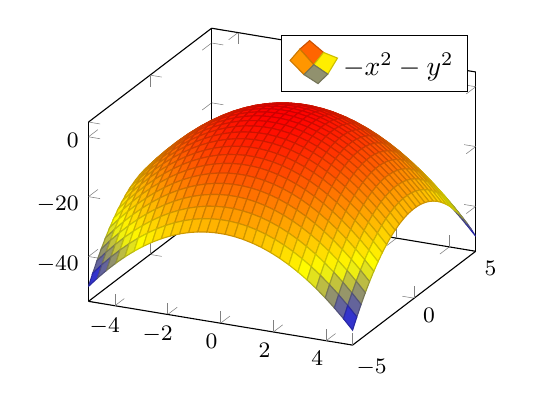
\begin{tikzpicture}
            \begin{axis}[samples=30,small]%
                \addplot3[surf]
                {- x^2 - y^2};
                \legend{$-x^2 - y^2$};
            \end{axis}
        \end{tikzpicture}
        \caption{Paraboloide, monomodale}
        \label{fig:intro-optim-hill-paraboloid}
        \vspace{4ex}
    \end{subfigure}
    \begin{subfigure}[b]{0.5 \textwidth}
        \centering
        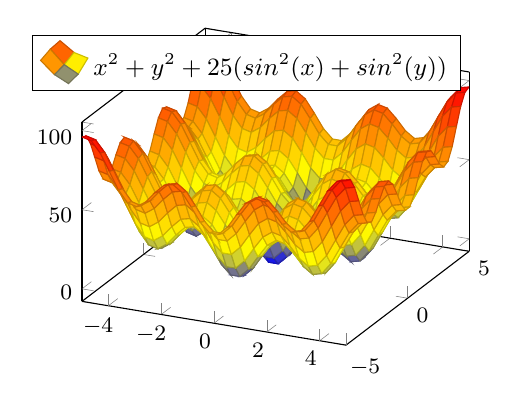
\begin{tikzpicture}
            \begin{axis}[samples=30,small]%
                \addplot3[surf] {25*(sin(deg(x))^2 + sin(deg(y))^2)+x^2+y^2};
                \legend{\small $x^2 + y^2 + 25(sin^2(x) + sin^2(y))$}
            \end{axis}
        \end{tikzpicture}
        \caption{``Eggcrate'', plurimodale}
        \label{fig:intro-optim-hill-egg}
        \vspace{4ex}
    \end{subfigure}
    \begin{subfigure}[b]{0.5 \textwidth}
        \centering
        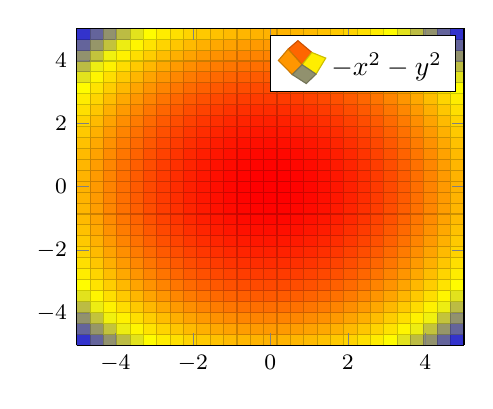
\begin{tikzpicture}
            \begin{axis}[samples=30,view={0}{90},small]%
                \addplot3[surf]
                {- x^2 - y^2};
                \legend{$-x^2 - y^2$};
            \end{axis}
        \end{tikzpicture}
        \caption{Paraboloide, monomodale}
        \label{fig:intro-optim-hill-paraboloid-contour}
    \end{subfigure}
    \begin{subfigure}[b]{0.5 \textwidth}
        \centering
        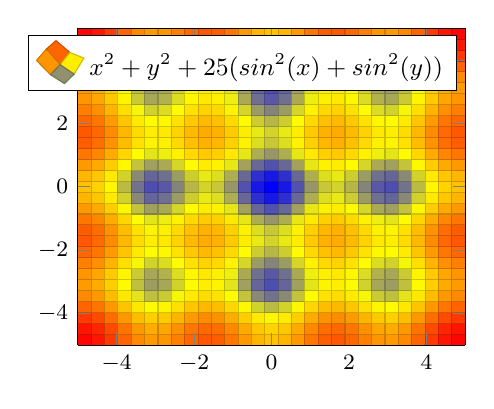
\begin{tikzpicture}
            \begin{axis}[samples=30,view={0}{90},small]%
                \addplot3[surf] {25*(sin(deg(x))^2 + sin(deg(y))^2)+x^2+y^2};
                \legend{\small $x^2 + y^2 + 25(sin^2(x) + sin^2(y))$}
            \end{axis}
        \end{tikzpicture}
        \caption{``Eggcrate'', plurimodale}
        \label{fig:intro-optim-hill-egg-contour}
    \end{subfigure}

    \label{fig:intro-optim-hill-functions}
    \caption{Esempi di funzione monomodale e plurimodale}
\end{figure}

D'altro canto, funzioni plurimodali\footnote{Una funzione plurimodale è una funzione con più di un ottimo locale. Non è detto che esista un unico ottimo globale} come ``Eggcrate'' rappresentato in \autoref{fig:intro-optim-hill-egg}, dove le tecniche citate precedentemente falliscono miseramente. Entrano quindi in gioco algoritmi di ricerca locale che ammettono, con un certo grado di libertà, di accettare un risultato peggiore di quello attuale, nella speranza di non rimanere intrappolati in un ottimo locale.

\subsection{Simulated Annealing}
\label{chap:intro-optim-sa}
Per cambiare e migliorare delle caratteristiche di un solido, in metallurgia viene utilizzata la tecnica della \textit{ricottura} (in inglese ``anneal''), dove i solidi come l'acciaio, bronzo o alluminio, vengono portati ad altissime temperature, per essere poi raffreddati ad una certa velocità chiamata \textit{cooling rate}, che determina le caratteristiche finali del metallo. Alle alte temperature, gli atomi si muovono molto velocemente e rompono le strutture cristalline che avevano formato precedentemente. Mano a mano che la temperatura cala, gli atomi rallentano, e si recristallizzano.

Analogamente, la tecnica matematica del \textit{simulated annealing} è un algoritmo di ricerca che utilizza la temperatura per riuscire a scappare da eventuali ottimi locali. Quando la temperatura è alta, l'algoritmo è meno propenso ad accettare nuovi soluzioni, anche se migliori. Mano a mano che la temperatura diminuisce, la probabilità che si accetti una soluzione migliore aumenta, fino al raggiuntimento della condizione di ottimalità, cioè quando la temperatura non può più scendere, ed il risultato non può che essere un ottimo locale.

\begin{algorithm}[h]
    $best \gets random()$ \\
    $T \gets 1.0$ \\
    $T_{min} \gets 0.0001$ \\
    $cooling\_rate \gets 0.9$ \\
    \While{$T > T_{min}$}{
        $new\_best = neighbour(best)$ \\
        $ap \gets acceptance\_probability(best, new\_best, T)$ \\
        \If{$ap > random()$}{
            $best \gets new\_best$
        }
        $T = T * cooling\_rate$
    }
    \label{algo:simulated-annealing}
    \caption{Simulated Annealing}
\end{algorithm}

Questa funzione però molto spesso fallisce, specie se si cerca di ottimizzare una funzione plurimodale come in \autoref{fig:intro-optim-hill-egg}.

\subsection{Particle Swarm Optimization}
\label{chap:intro-optim-pso}
Un'altra tecnica di ricerca dell'ottimo è quella del \textit{particle swarm optimization}. Questo algoritmo iterativo nasce inizialmente come simulazione del comportamente sociale di stormi di uccelli che si sincronizzano in volo, o un branco di pesci alla ricerca di cibo \cite{pso}: membri individuali del branco possono trarre vantaggio dalle scoperte ed esperienze passate di tutti gli altri membri durante la ricerca del cibo, un vantaggio che può rivelarsi decisivo per superare la competizione. Questa è un'ipotesi fondamentale per poter definire il \textit{particle swarm optimization}.

Nell'algoritmo, il branco di pesci viene sfruttato come analogia per lo \textit{swarm} (rappresentato in \autoref{fig:intro-optim-pso-swarm}), che indica l'insieme degli elementi appartenenti ad una popolazione, questi indicati come \textit{particelle} dello swarm.

\begin{figure}[!h]
    \begin{minipage}{0.5 \textwidth}
        \centering
        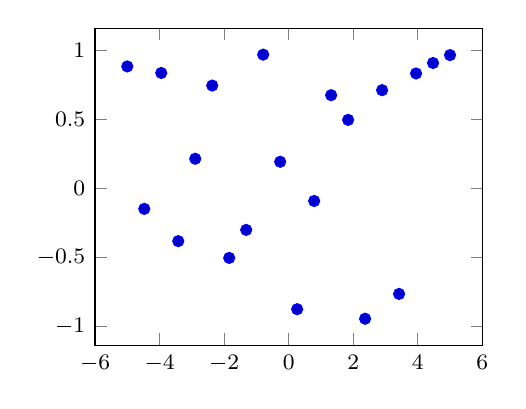
\begin{tikzpicture}
            \begin{axis}[scatter/classes={a=mark=o},small]%
                \addplot+[scatter,only marks,samples=20] {rand};
            \end{axis}
        \end{tikzpicture}
        \caption{\small Esempio di swarm}
        \label{fig:intro-optim-pso-swarm}
    \end{minipage}
    \begin{minipage}{0.5 \textwidth}
        \centering
        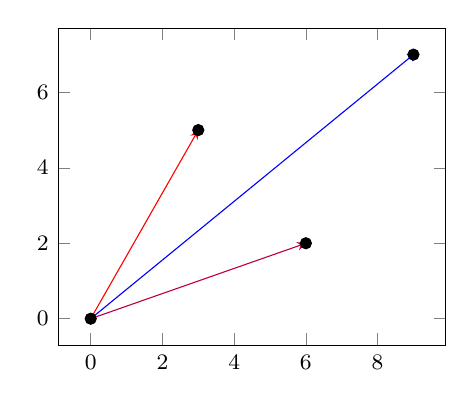
\begin{tikzpicture}
            \begin{axis}[small]%
                \draw[red,-stealth]
                    (axis cs:0,0) 
                    -- % = line-to
                    (axis direction cs:3,5);
                \draw[blue,->]
                    (axis cs:0,0)
                    --
                    (axis direction cs:9,7);
                \draw[purple,-stealth,solid]
                    (axis cs:0,0)
                    --
                    (axis direction cs:6,2);
                \addplot [only marks,mark=*]
                    coordinates { (0,0) (3,5) (6,2) (9,7) };
            \end{axis}
            \end{tikzpicture}
        \caption{\small Somma vettoriale tra $p_i$ e $g$}
        \label{fig:intro-optim-pso-sum}
    \end{minipage}
\end{figure}

Ad ogni iterazione, la posizione di ogni particella viene aggiornata per ogni dimensione del problema, basandosi sulla migliore posizione della particella $p_{i}$ e sulla migliore posizione globale dello swarm $g$ (in \autoref{fig:intro-optim-pso-sum} si vede un esempio di questa combinazione, dove la posizione finale del vettore è data dalla combinazione di due valori). Questa combinazione dei due valori migliori risolve il problema di rimanere intrappolati in un ottimo locale che presentano gli algoritmi visti nella \autoref{chap:intro-optim-hill}. Con il proseguire dell'algoritmo sarà possibile osservare che le singole particelle mano a mano convergono verso un ottimo locale, o di più, se la funzione da ottimizzare è multimodale (come in \autoref{fig:intro-optim-hill-egg}). È possibile inoltre introdurre la \textit{velocità} come parte dell'algoritmo, al fine di influire su quanto velocemente una particella si muove verso la soluzione, che in algebra vettoriale si traduce nella modifica del modulo del vettore di spostamento.

\begin{algorithm}[!h]
    \caption{Particle Swarm Optimization}
    $n = $ numero particelle \\
    $m = $ numero dimensioni dello spazio di ricerca \\
    \For{$i \gets 1$ \KwTo $n$}{
        $x_i \sim U(b_{low}, b_{up})$ \Comment{Inizializzo ogni particella con un valore random nel mio spazio di ricerca, delimitato da un lower bound $b_{low}$ ed un $b_{up}$}
        $p_i \gets x_i$ \Comment{Inizializzo la posizione migliore della particella alla sua posizione iniziale}
        \If{$f(p_i) > f(g)$}{
            $g \gets p_i$ \Comment{Aggiorno la posizione migliore globale}
        }
        $v_i \sim U(-\abs{b_{up} - b_{low}}, \abs{b_{up} - b_{low}})$ \Comment{Inizializzo la velocità iniziale della particella}
    }
    \While{criterio di terminazione non soddisfatto} {
        \For{$i \gets 1$ \KwTo $n$} {
            \For{$d \gets 1$ \KwTo $m$} {
                $r_p, r_g \sim U(0, 1)$ \Comment{Parametri di casualità}
                $v_{i, d} \gets \omega v_{i, d} + \phi_p r_p (p_{i, d} - x_{i, d}) + \phi_g r_g (g_d - x_{i, d})$ \Comment{Aggiorno la velocità della particella}
                $x_i \gets x_i + v_i$ \Comment{Aggiorno la posizione della particella}
                \If{$f(x_i) > f(p_i)$}{
                    $p_i \gets x_i$ \Comment{Aggiorno la posizione migliore della particella}
                    \If{$f(p_i) > f(g)$}{
                        $g \gets p_i$ \Comment{Aggiorno la posizione migliore dello swarm}
                    }
                }
            }
        }
    }
    \label{algo:pso}
\end{algorithm}

\section{Nozioni Extra}
\label{chap:intro-extra}
In questa sezione verranno introdotti dei concetti aggiuntivi che non rientrano nelle sezioni sopracitate, e le cui basi si assumono essere già presenti per la comprensione degli stessi. Queste nozioni verranno utilizzate nei capitoli successivi per complementare la spiegazione di modelli, termini o algoritmi.

\subsection{Catena di Markov}
\label{chap:intro-extra-markov}
In teoria probabilistica, una \textit{Catena di Markov} è un modello stocastico che descrive una sequenza di possibili eventi la cui probabilità dei singoli eventi dipende solo ed unicamente dallo stato dell'evento che lo precede. Questa definizione si traduce nell'assunzione che gli stati passati e futuri di ogni evento sono indipendenti rispetto alla storia di tutti gli eventi già avvenuti all'interno della catena.

Il modello è strutturato come una \textit{macchina a stati finiti}, dove i rami che collegano uno stato ad un altro hanno un valore numero associato, chiamato la \textit{probabilità di transizione}, che indica quanto è probabile passare allo stato di destinazione.

\begin{figure}[h]
    \centering
    \begin{tikzpicture}[start chain = going right,-Triangle, every loop/.append style = {-Triangle}]
        \node[state, on chain]  (0) {A};
        \node[state, on chain]  (1) {B};
        \node[state, on chain]  (2) {C};
        \node[state, on chain]  (3) {D};

        \draw
            (0) edge[bend left] node[above] {$0.3$} (1)
            (1) edge[bend left] node[below] {$0.7$} (0)
            (1) edge[bend left] node[above] {$0.2$} (2)
            (2) edge[bend left] node[below] {$0.7$} (1)
            (2) edge[bend left] node[above] {$0.2$} (3)
            (3) edge[bend left] node[below] {$0.4$} (2)
            ;

        \foreach \i in {1,...,2}
          \draw  (\i) edge[loop below] node[below] {$0.1$} (\i);

        \draw   (0)  edge[loop left] node[left] {$0.7$} (0);
        \draw   (3)  edge[loop right] node[right] {$0.6$} (3);
     \end{tikzpicture}
     \caption{Esempio di catena di Markov}
    \label{fig:intro-markov-chain}
\end{figure}

Una catena di Markov può essere vista anche come una sequenza di variabili aleatorie $X_0, X_1, X_2, \dots$ che soddisfano la proprietà di indipendenza. Questa soddisfacibilità è definita come \textit{Proprietà di Markov}:

\begin{equation}
    P(X_n = i_n | X_{n - 1} = i_{n - 1}) = P(X_n = i_n | X_0 = i_0, X_1 = i_1, \dots, X_{n - 1} = i_{n - 1})
    \label{eq:intro-markov-property}
\end{equation}

Le probabilità di transizione in un dato tempo $t$ per ogni stato della catena possono essere rappresentate come una matrice $P_t$, denominata \textit{matrice di transizione} e definita come segue:

\begin{equation}
    (P_t)_{i,j} = \mathbb{P} (X_{t + 1} = j | X_t = i)
    \label{intro-extra-markov-matrix}
\end{equation}

Questo significa che ogni riga della matrice è un \textit{vettore di probabilità}, e la somma dei suoi elementi è sempre $1$. 

Una matrice di transizione $P_t^(k) = P_t \cdot P_{t + 1} \cdots P_{t + k - 1}$ soddisfa quindi: 

\begin{equation}
    P_t^{(k)} = \begin{pmatrix}
        \mathbb{P}(X_{t+k} = 1 \mid X_t = 1) & \mathbb{P}(X_{t+k} = 2 \mid X_t = 1) & \dots & \mathbb{P}(X_{t+k} = n \mid X_t = 1) \\
        \mathbb{P}(X_{t+k} = 1 \mid X_t = 2) & \mathbb{P}(X_{t+k} = 2 \mid X_t = 2) & \dots & \mathbb{P}(X_{t+k} = n \mid X_t = 2) \\
        \vdots & \vdots & \ddots & \vdots \\
        \mathbb{P}(X_{t+k} = 1 \mid X_t = n) & \mathbb{P}(x_{t+k} = 2 \mid X_t = n) & \dots & \mathbb{P}(X_{t+k} = n \mid X_t = n)
        \end{pmatrix}.
    \label{eq:intro-extra-markov-property}
\end{equation}

Nell'esempio in \autoref{fig:intro-markov-chain} la matrice di transizione a $k = 0$ è come segue:
\begin{equation}
    P_t^0 = \begin{pmatrix}
        0.7 & 0.3   & 0     & 0 \\
        0.7 & 0.1   & 0.2   & 0 \\
        0   & 0.7   & 0.1   & 0.2 \\
        0   & 0     & 0.4   & 0.6
    \end{pmatrix}
    \label{eq:intro-markov-tranmat}
\end{equation}

\subsubsection{Catena di Markov: Variante Monte Carlo (MCMC)}
\label{chap:intro-extra-markov-mc}
Il metodo \textit{Monte Carlo} in statistica si basa sul campionamento casuale per ottenere dei risultati. Un esempio del loro utilizzo è dato dal calcolo dell'area di una funzione complessa: vengono generati $n$ punti casuali, e si calcola quanti di questi rientrano all'interno della funzione della quale vogliamo calcolare l'area. Il numero di questi punti che ricade in questa categoria ci fornisce un grado di approssimazione proporzionale al numero di punti che generiamo per ottenere il risultato finale: più punti generiamo, più è accurata la stima dell'area, o più in generale, di qualunque cosa stiamo cercando di approssimare.

Volendo ad esempio stimare una distribuzione a posteriori\footnote{Distribuzione di una variabile aleatoria condizionata a delle informazioni rilevanti su di essa} è possibile utilizzare una variante della Catena di Markov sfruttando le proprietà aleatorie del metodo Monte Carlo: la tecnica così ottenuta è definita una \textit{Monte Carlo Markov Chain} (MCMC). Ogni valore generato è aleatorio, ma le scelte fatte per generare i valori successivi sono limitate dallo stato corrente e dalla distribuzione dei valori attuali. Una MCMC quindi può essere paragonata ad un cammino aleatorio\footnote{Modello matematico che descrive un processo stocastico come una successione di step aleatori all'interno di uno spazio matematico (e.g. $\mathbb{Z}$)} che con l'aumentare delle iterazioni converge alla distribuzione (o modello matematico) che si vuole stimare.

\subsection{Likelihood}
\label{chap:intro-extra-lh}
Uno dei problemi della genomica (ma anche di altri campi, come la linguistica \cite{phylogenylinguistical}) è quello di ricostruire un albero filogenetico partendo da dati raccolti di caratteri appartenenti una popolazione. I dati in questione seguono il modello di sostituzione (\autoref{chap:intro-models}) ed i tratti possono essere qualunque aspetto della popolazione, come altezza, peso, capacità di volare o di respirare sott'acqua. Nel presente lavoro, la popolazione presa in analisi sono cellule, ed i tratti considerati sono le mutazioni acquisite, ed il problema si può interpretare come la ricerca del migliore albero filogenetico che meglio rappresenta il modello di sostituzione. Per stabilire come un albero è \textit{migliore} di un altro, viene definita una funzione di \textit{likelihood}, che esprime appunto quanto è probabile un particolare set di parametri stastistici (nel nostro caso la configurazione dei nodi dell'albero inferito) data il modello di sostituzione iniziale. Supponendo di aver generato un albero $T$ con $n$ nodi, un nodo per ogni mutazione, e ad ogni foglia può essere associata una cellula. Le cellule così assegnate avranno una serie di caratteri, che vengono acquisiti o persi una volta per ogni nodo padre.

\begin{figure}[!h]
    \begin{subfigure}[b]{0.5 \textwidth}
        \centering
        \begin{tabular}{*{4}{c}}
            a & b & c & d \\ \midrule \midrule
            1 & 0 & 0 & 0 \\
            0 & 1 & 0 & 0 \\
            1 & 0 & 1 & 0 \\
            1 & 0 & 1 & 1
        \end{tabular}
        \caption{Modello di sostituzione}
        \label{fig:intro-extra-lh-tree-matrix}
    \end{subfigure}
    \begin{subfigure}[b]{0.5 \textwidth}
        \centering
        \begin{forest}
            for tree = {grow'=0,draw}, forked edges
            [root,
                [a, [c, [d]] ]
                [b]
            ]
        \end{forest}
        \caption{Esempio di albero inferito}
        \label{fig:intro-extra-lh-tree-model}
    \end{subfigure}
    \caption{}
    \label{fig:intro-extra-lh-tree}
\end{figure}

Il calcolo della likelihood $\mathcal{L}$ si basa sulla probabilità condizionata della configurazione attuale dell'albero $T$ dato il modello di sostituzione in input $M$, con $n$ righe (una per ogni cellula) e $m$ colonne (una per ogni mutazione), che si traduce in termini generali nella formula che segue:

\begin{equation}
    \mathcal{L}(T) = \mathcal{L}(1) \cdot \mathcal{L}(2) \cdots \mathcal{L}(n) = P(M | T) = \prod_{j = 1}^{m} P(M_j | T)
    \label{eq:intro-extra-lh-formula}
\end{equation}

Spesso è utile riportare la somma logaritmica delle likelihood ad ogni posizione, poiché le probabilità condizionate di ogni nodo si traducono in numeri molto piccoli. La formula per il calcolo della \textit{logaritmic likelihood} si traduce quindi come segue:

\begin{equation}
    \ln \mathcal{L} = \ln \mathcal{L}(1) + \ln \mathcal{L}(2) + \ln \mathcal{L}(n) = \sum_{j = 1}^m \ln \mathcal{L}(j)
    \label{eq:intro-extra-lh-log}
\end{equation}

\subsection{Matching}
Nella teoria dei grafi un \textit{matching} $M$ è definito come un sottoinsieme di coppie di nodi di un grafo $G = (V, E, w)$ tale per cui ogni coppia non è adiacente ad un altra, e nessuna coppia è un loop; ciò significa che nessuna coppia condivide un nodo.

\begin{figure}[h]
    \centering
    \begin{forest}
        for tree = {grow'=0,draw}, forked edges
        [,
            [, edge=red]
            [, [, [, [, [, ]]]]]
            [, [, edge=red [, ]]]
            [, [, [, edge=red]]]
        ]
    \end{forest}
    \caption{Esempio di matching}
    \label{fig:intro-extra-matching}
\end{figure}

\subsubsection{Maximum Weight Matching}
Dato un matching $M$ 